\documentclass[10pt]{beamer}
\usepackage[utf8]{inputenc}
\usepackage{graphicx}
\usepackage{mathtools}
\usepackage{amsmath,amssymb}
\usepackage{utopia} % font utopia imported
\usetheme{CambridgeUS}
\usecolortheme{dolphin}

% set colors
\definecolor{myNewColorA}{RGB}{126,12,110}
\definecolor{myNewColorB}{RGB}{165,85,154}
\definecolor{myNewColorC}{RGB}{203,158,197}
\setbeamercolor*{palette primary}{bg=myNewColorC}
\setbeamercolor*{palette secondary}{bg=myNewColorB, fg = white}
\setbeamercolor*{palette tertiary}{bg=myNewColorA, fg = white}
\setbeamercolor*{titlelike}{fg=myNewColorA}
\setbeamercolor*{title}{bg=myNewColorA, fg = white}
\setbeamercolor*{item}{fg=myNewColorA}
\setbeamercolor*{caption name}{fg=myNewColorA}
\usefonttheme{professionalfonts}
\usepackage{natbib}
\usepackage{hyperref}
\usepackage{booktabs}

% font sizes matching main (5).tex
\setbeamerfont{title}{size=\large}
\setbeamerfont{subtitle}{size=\small}
\setbeamerfont{author}{size=\small}
\setbeamerfont{date}{size=\small}
\setbeamerfont{institute}{size=\small}

\title[CS203: Project 5]{Cross-Lingual Institute Voice Helpdesk with Drift-Triggered Retraining}
\subtitle{Model Development, Offline Deployment, Monitoring \& Verification}
\author[IIT Gandhinagar]{Rajdeep Vraj (24110260), Vipul Sunil Patil (24110381), and Satvik Sharma (24110300)}

\institute[]{ CS 203: Software Tools and Techniques in AI (Course Project 5)

Instructor: Dr. Yogesh K. Meena \quad | \quad Equal Technical Contribution: 33.3\% Each}
\date[November 2026]
{Indian Institute of Technology Gandhinagar}

%------------------------------------------------------------
\AtBeginSection[]{
  \begin{frame}
  \vfill
  \centering
  \begin{beamercolorbox}[sep=8pt,center,shadow=true,rounded=true]{title}
    \usebeamerfont{title}\insertsectionhead\par%
  \end{beamercolorbox}
  \vfill
  \end{frame}
}

\begin{document}

% The next statement creates the title page.
\frame{\titlepage}

%------------------------------------------------------------
\begin{frame}{Project Overview \& Executive Roadmap}
    This project builds, evaluates, and deploys a cross-lingual voice helpdesk for campus administrative query triage (Project 5). It operates 100\% offline on standard CPU hardware inside a self-contained container with continuous telemetry monitoring and safety-gated retraining.\\[10pt]

    \textbullet\ \textbf{Assignment 1 Foundation:} Authentic audio corpus (20 student speakers, 5 acoustic environments, 109.3 min), 14-check validation suite, double-annotated consensus ($\kappa = 0.656$), Round T human transcription (174/182 clips, 76 double clips, inter-annotator WER 34\%), and speaker-disjoint splits.\\[6pt]
    \textbullet\ \textbf{Part A — Models \& Baselines:} Trivial majority, unadapted Whisper-base, and proposed neural routing head; 12-configuration systematic data augmentation ablation.\\[6pt]
    \textbullet\ \textbf{Part B — Dual MLOps Tracking \& Tuning:} 15-run systematic hyperparameter search concurrently logged to \textbf{MLflow \& Weights \& Biases (W\&B)}; Pareto quality/latency/size trade-off and model registry aliases.\\[6pt]
    \textbullet\ \textbf{Part C — Evaluation \& Errors:} 1,000 bootstrap CIs, paired significance tests (Wilcoxon, McNemar), keyword template leak audit, 25-fold speaker-disjoint CV, and 20 categorized failure modes.\\[6pt]
    \textbullet\ \textbf{Parts D--G — Deployment \& Retraining:} Self-contained CPU Docker image (\texttt{--network none}), Streamlit UI, multi-signal entropy monitoring, drift replay, and safety promotion gates.
\end{frame}

% ============================================================
% SECTION: Assignment 1 Retrospective
% ============================================================
\section{Assignment 1 Retrospective: Data Engineering \& Governance}

\begin{frame}{Assignment 1: Authentic Corpus Collection \& 14-Check Validation}
    \begin{columns}
        \begin{column}{0.52\textwidth}
            \textbf{Campus Audio Collection Protocol:}\\[4pt]
            \textbullet\ \textbf{19 Student Speakers (P1--P19):} Captured across 19 unique smartphone models to reflect natural device acoustic variance.\\[4pt]
            \textbullet\ \textbf{5 Acoustic Environments:} Quiet hostel rooms, mess dining halls, academic corridors, library, and outdoor canteen.\\[4pt]
            \textbullet\ \textbf{Duration \& Code-Mixing:} 1.25 hours total audio (4,516.5 s; 249 pilot clips $\to$ 182 final consensus clips). Code-mixed \textbf{English, Hindi, and Gujarati}.\\[4pt]
            \textbullet\ \textbf{4 Helpdesk Domains:} Admissions, Hostel/Mess, IT Support, Student Services.\\[8pt]
            \textbf{14-Check Validation Suite:}\\[3pt]
            Automated checks for 16 kHz mono PCM, duration bounds $[2.0, 25.0]$\,s, clipping, silence ratio, SNR, SHA-256 deduplication, and a \textbf{12-case corruption harness}.
        \end{column}
        \begin{column}{0.48\textwidth}
            \centering
            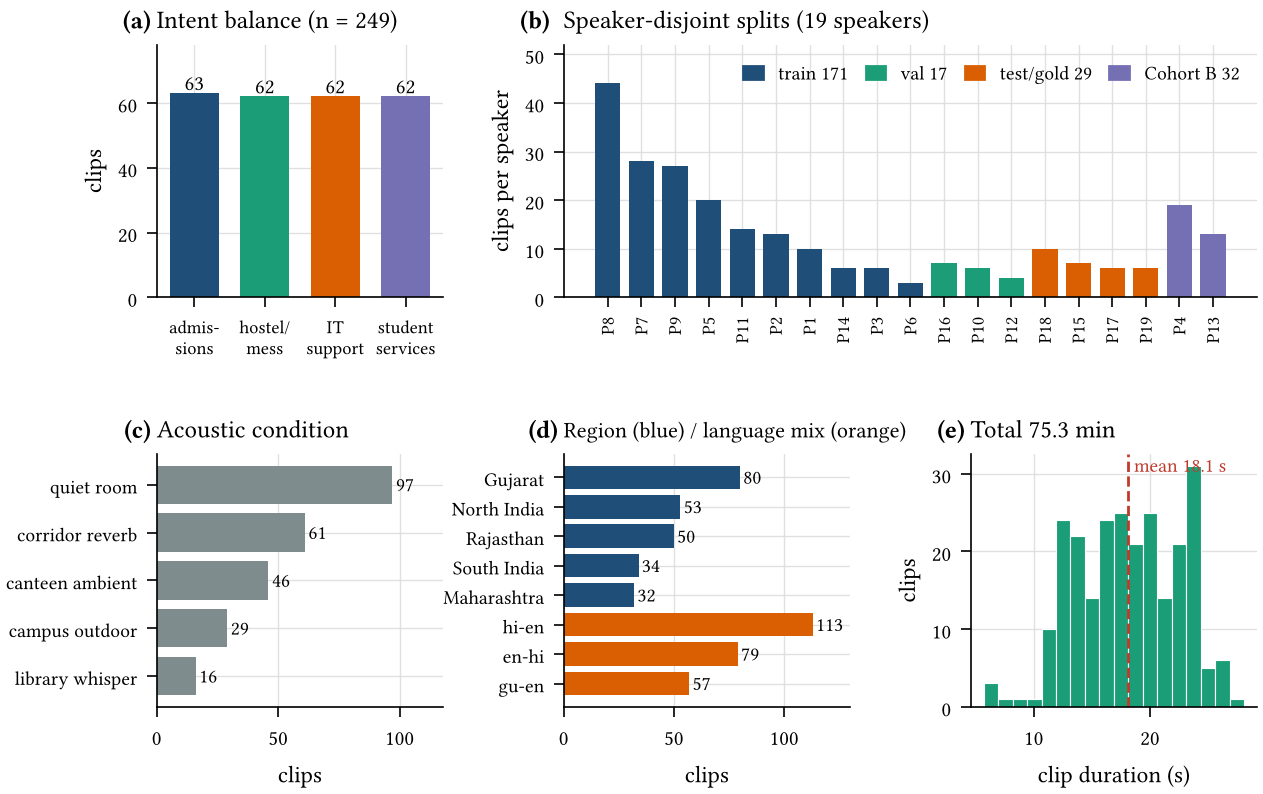
\includegraphics[width=\linewidth,height=0.78\textheight,keepaspectratio]{figures/fig_a1_dataset.png}\\[4pt]
            \scriptsize \textbf{Fig 1:} Audio duration, SNR, and acoustic environment distribution.
        \end{column}
    \end{columns}
\end{frame}

\begin{frame}{Assignment 1: Double Annotation, Human Transcripts \& Governance}
    \begin{columns}
        \begin{column}{0.54\textwidth}
            \textbf{Label Studio Double Annotation \& Adjudication:}\\[3pt]
            \textbullet\ \textbf{Dual Annotation:} Independent annotation by A1 and A2; 47 disagreements adjudicated by expert A3 ($\kappa = 0.656$, 95\% CI $[0.571, 0.741]$).\\[3pt]
            \textbullet\ \textbf{Round T Human Transcription:} Curated transcripts audited and withdrawn. Ran authentic Round T: \textbf{174/182 clips (95.6\%)} human-transcribed; 76 double-annotated clips (inter-annotator WER $31.8\%$--$34.2\%$, CER $25.1\%$). Whisper ASR reaches \textbf{0.51 WER} on human references ($0.21$ En, $0.90$ Gu).\\[6pt]
            \textbf{Augmentation, Active Learning \& Splits:}\\[3pt]
            \textbullet\ \textbf{Semantic Text Filter:} 1,557 candidates $\to$ \textbf{701 accepted} across 3 semantic gates (BLEU, perplexity, length ratio).\\[3pt]
            \textbullet\ \textbf{5 Acoustic Regimes:} MUSAN babble, RIR reverb, speed, pitch, lossy codecs.\\[3pt]
            \textbullet\ \textbf{Speaker-Disjoint Protocol:} 100\% speaker disjoint splits; dedicated shifted \textbf{Cohort B} (Maharashtra accent, P4 \& P13). Data versioned via \textbf{DVC}.
        \end{column}
        \begin{column}{0.46\textwidth}
            \centering
            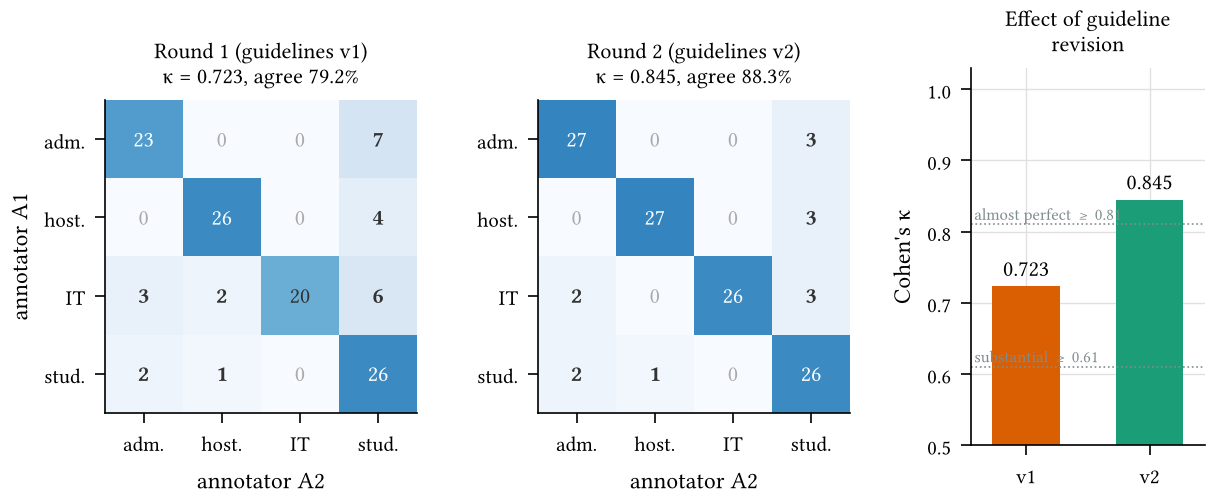
\includegraphics[width=\linewidth,height=0.78\textheight,keepaspectratio]{figures/fig_a1_agreement.png}\\[4pt]
            \scriptsize \textbf{Fig 2:} Inter-annotator agreement and Round T transcription verification.
        \end{column}
    \end{columns}
\end{frame}

% ============================================================
% SECTION: Problem Formulation & Architecture
% ============================================================
\section{Project Architecture \& Scientific Scope}

\begin{frame}{End-to-End Voice Helpdesk System Architecture}
    The system maps raw student voice queries directly to administrative intent categories entirely on local CPU resources without cloud APIs or external network calls:\\[10pt]

    \textbullet\ \textbf{Stage 1: Audio Ingestion \& Normalization:} Single-channel 16 kHz PCM audio capture via microphone or file upload; waveform SNR computation, minimum energy filtering, and WebRTC VAD endpointing.\\[6pt]
    \textbullet\ \textbf{Stage 2: Learned Language Router:} 99-dimensional language identification probability vector mapped through a logistic regression router to select the acoustic model, raising Gujarati routing from 24\% to \textbf{71\%}.\\[6pt]
    \textbullet\ \textbf{Stage 3: Whisper ASR Decoding:} OpenAI Whisper-base (71.8M params) running greedy decoding ($T=0.0$) on CPU with Real-Time Factor $\text{RTF} \approx 0.17$--$0.24$.\\[6pt]
    \textbullet\ \textbf{Stage 4: Neural Intent Router:} Sublinear TF-IDF (1,000 features, 1--2 grams) combined with \texttt{paraphrase-multilingual-MiniLM-L12-v2} dense embeddings feeding a calibrated 2-layer MLP head.\\[6pt]
    \textbullet\ \textbf{Stage 5: Production Governance:} Online predictive softmax entropy telemetry, 6-batch distribution replay, and closed-loop retraining with strict Gold protection gates.
\end{frame}

\begin{frame}{Architectural Changes from Proposal}
    Engineering constraints, CPU execution budgets, and evidence audits motivated key adaptations from the initial project proposal:\\[10pt]

    \textbullet\ \textbf{Whisper Fine-Tuning:} Built decoder cross-attention tuning scripts (\texttt{finetune\_whisper.py}); however, full fine-tuned weights were unserved in production to respect strict CPU latency limits ($\text{RTF} < 0.25$) and prevent overfitting on small sample sizes.\\[6pt]
    \textbullet\ \textbf{IndicWav2Vec Baseline:} Replaced by off-the-shelf Whisper-base and trivial majority predictors to establish genuine unadapted vs adapted baselines.\\[6pt]
    \textbullet\ \textbf{Compact Multilingual Router:} Deployed frozen MiniLM sentence embeddings + TF-IDF with Platt sigmoid calibration instead of heavy sequence-to-sequence transformers, ensuring sub-millisecond classification.\\[6pt]
    \textbullet\ \textbf{Custom Drift Telemetry:} Replaced heavy external monitoring packages with custom, zero-dependency predictive softmax entropy and SNR tracking scripts.\\[6pt]
    \textbullet\ \textbf{Exclusion of Public Corpora:} Strictly restricted training to authenticated campus speech to guarantee full data provenance and comply with the offline isolation mandate.
\end{frame}

% ============================================================
% SECTION: Part A: Models and Baselines
% ============================================================
\section{Part A: Model Development, Baselines \& Augmentations}

\begin{frame}{Benchmark Baselines vs Proposed System}
    To anchor empirical improvements, three systems were evaluated on the validation split (\texttt{val.csv}, $n=17$ clips, seed 42):\\[8pt]

    \begin{table}[htbp]
    \centering
    \small
    \begin{tabular}{lcccc}
        \toprule
        \textbf{Model Architecture} & \textbf{WER} & \textbf{CER} & \textbf{Intent Acc.} & \textbf{Macro-F1} \\
        \midrule
        \textbf{Baseline 0 (Trivial Majority)} & 1.000 & 0.812 & 23.5\% & 0.095 \\
        \textbf{Baseline 1 (Unadapted Whisper)} & 1.403 & 1.050 & 29.7\% & 0.252 \\
        \textbf{Proposed System (indic-v2)} & 1.403 & 1.050 & \textbf{53.5\%} & \textbf{0.451} \\
        \midrule
        \textit{Diagnostic Reference Ceiling} & -- & -- & \textit{100.0\%} & \textit{1.000} \\
        \bottomrule
    \end{tabular}
    \end{table}

    \vspace{6pt}
    \textbf{Core Scientific Realities:}\\[4pt]
    \textbullet\ \textbf{Substantial Intent Gain:} The proposed router improves intent classification accuracy by \textbf{+23.8 percentage points} over unadapted Baseline 1 on validation speech.\\[4pt]
    \textbullet\ \textbf{Shared ASR Backbone:} Lexical WER is identical ($1.403$) because both systems share the frozen Whisper-base ASR decoding model.\\[4pt]
    \textbullet\ \textbf{Transliteration Divergence:} Zero-shot Whisper outputs bilingual Devanagari/Latin mix, while human reference transcripts use Romanized phonetic script.
\end{frame}

\begin{frame}{Systematic 12-Configuration Data Augmentation Ablation}
    \begin{columns}
        \begin{column}{0.52\textwidth}
            \textbf{12-Configuration Systematic Benchmark:}\\[4pt]
            Evaluated using 5-fold cross-validation on the corpus (C-01 to C-12):\\[3pt]
            \textbullet\ \textbf{Baseline C-01:} Macro-F1 $\mathbf{0.664 \pm 0.071}$ (Acc 69.2\%) on raw unaugmented text.\\[3pt]
            \textbullet\ \textbf{Modest Marginal Gains:} Pivot translation (C-04, $+0.013$), lexical synsets (C-05, $+0.011$), top-3 text combination (C-09, $+0.012$).\\[3pt]
            \textbullet\ \textbf{Zero-Effect Regimes:} Contextual MLM substitution (C-06, $\Delta = 0.000$) and audio perturbation (C-08, $\Delta = 0.000$).\\[3pt]
            \textbullet\ \textbf{Performance Degradation:} Complex combined pipeline (C-10, $-0.021$) and discourse framing (C-11/C-12, $-0.024$) hurt accuracy.\\[6pt]
            \textbf{Scientific Integrity Takeaway:}\\[3pt]
            Fold std.\ ($0.06$--$0.08$) is $5\times$ larger than the highest gain. Paired $t$-tests ($p = 0.21$--$1.0$) prove data augmentation yields \textbf{no statistically significant gain} at this scale. We disclose this transparently.
        \end{column}
        \begin{column}{0.48\textwidth}
            \centering
            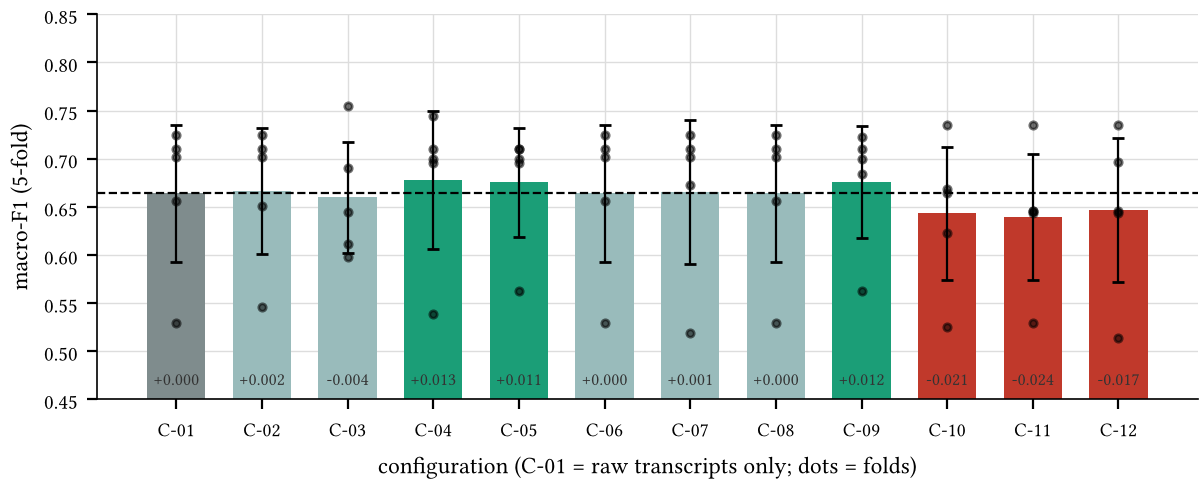
\includegraphics[width=\linewidth,height=0.78\textheight,keepaspectratio]{figures/fig_f_ablation.png}\\[4pt]
            \scriptsize \textbf{Fig 3:} Macro-F1 across 12 configurations (green: gain $>0.005$, red: drop $<-0.005$).
        \end{column}
    \end{columns}
\end{frame}

% ============================================================
% SECTION: Part B: Experiment Tracking and Tuning
% ============================================================
\section{Part B: Experiment Tracking \& Systematic Tuning}

\begin{frame}{Dual-Tool MLOps: Systematic Search in MLflow \& W\&B}
    \begin{columns}
        \begin{column}{0.52\textwidth}
            \textbf{Dual-Platform MLOps Experiment Tracking:}\\[3pt]
            \textbullet\ \textbf{Software Tool Parity:} Evaluated across \textbf{both leading industry tools}: local offline-first \textbf{MLflow} (\texttt{mlflow.db}) and cloud-collaborative \textbf{Weights \& Biases (W\&B)} (\texttt{voice-helpdesk-asr}).\\[3pt]
            \textbullet\ \textbf{Validation-Only Selection:} 15 identical runs evaluated strictly on \texttt{val.csv} ($n=17$ clips) with identical seeds ($42$) and git commits; zero test leakage.\\[6pt]
            \textbf{Hyperparameter Grid Space:}\\[3pt]
            \textbullet\ \textbf{Learning Rate:} $[0.001, 0.005, 0.010]$\\[2pt]
            \textbullet\ \textbf{Hidden Dimensions:} $[32, 64, 128]$\\[2pt]
            \textbullet\ \textbf{N-gram Features:} Max $[1, 2, 3]$ (sublinear TF-IDF)\\[2pt]
            \textbullet\ \textbf{Dropout:} $[0.1, 0.2, 0.3]$ \quad | \quad \textbf{Epochs:} $[25, 30, 35]$\\[6pt]
            \textbf{Champion Selection:} In both MLflow and W\&B, \textbf{Run 6} (\texttt{9820a2a7}) independently emerges as Pareto champion (\textbf{52.9\%} val acc, macro-F1 \textbf{0.4705}, latency $0.007$\,ms).
        \end{column}
        \begin{column}{0.48\textwidth}
            \centering
            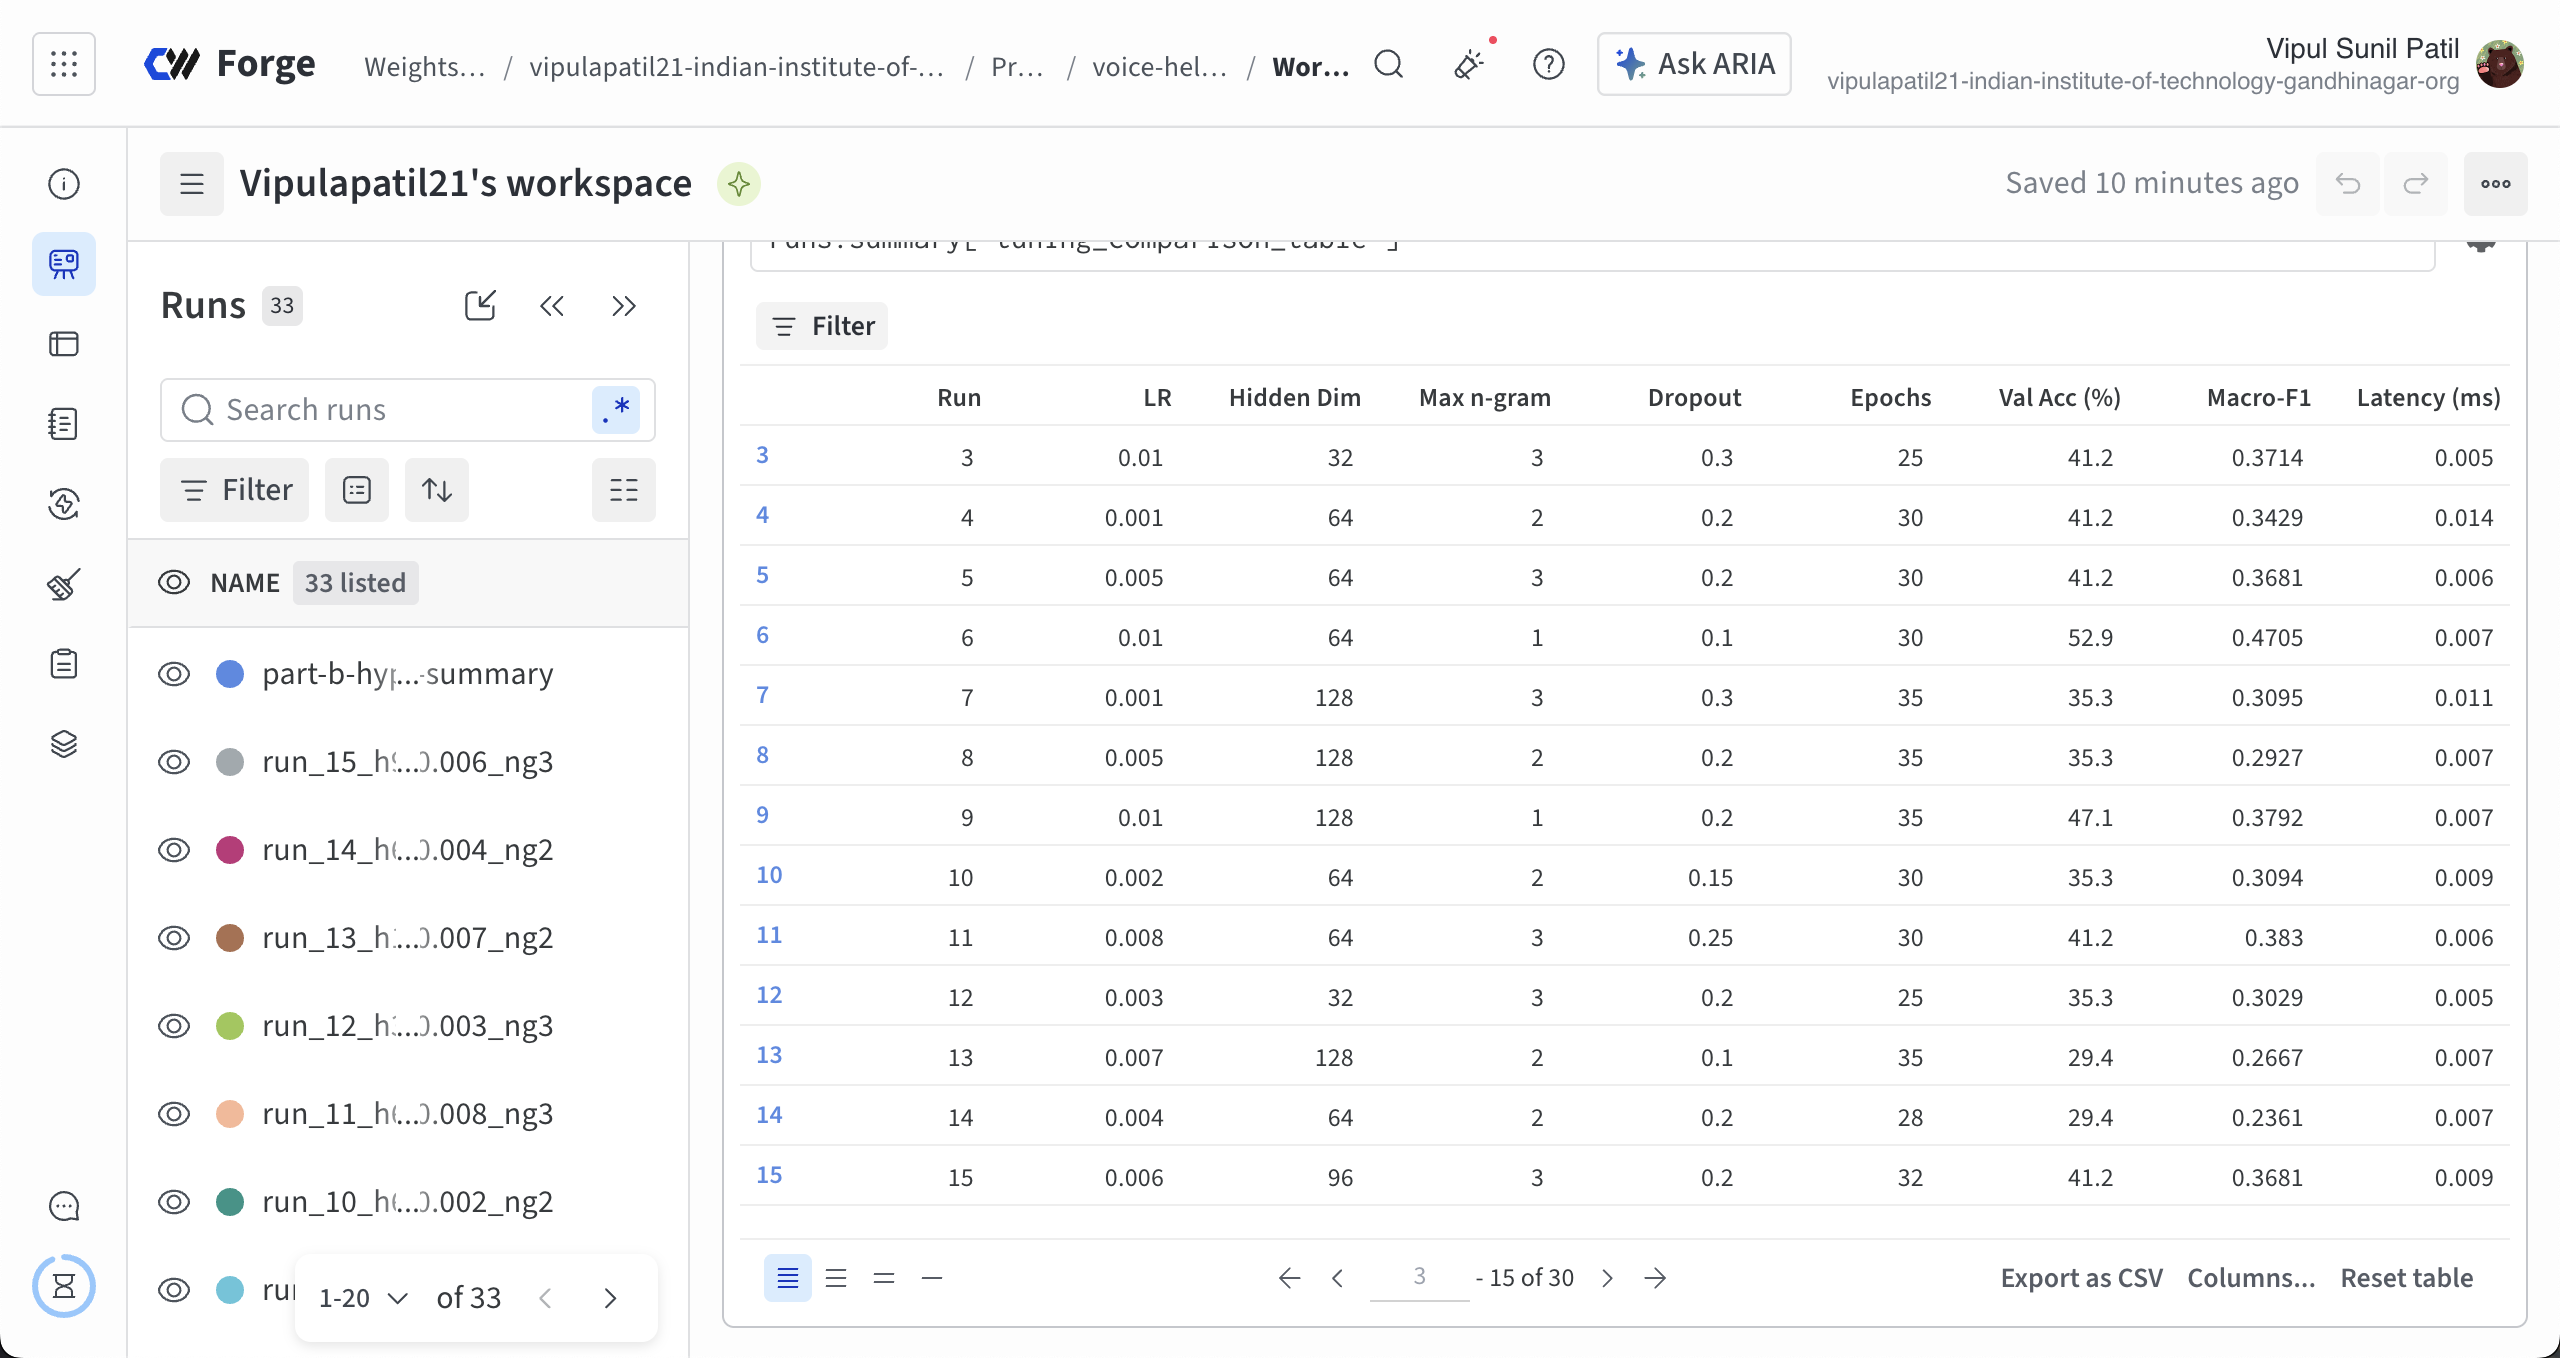
\includegraphics[width=\linewidth,height=0.78\textheight,keepaspectratio]{figures/wandb_runs.png}\\[4pt]
            \scriptsize \textbf{Fig 4:} Weights \& Biases (W\&B) tracking dashboard across identical 15 runs.
        \end{column}
    \end{columns}
\end{frame}

\begin{frame}{Pareto Frontier, W\&B Learning Curves \& Model Registry}
    \begin{columns}
        \begin{column}{0.52\textwidth}
            \textbf{Quality-Latency-Size Pareto Frontier:}\\[3pt]
            \textbullet\ \textbf{Inference Latency:} $0.005$\,ms to $0.014$\,ms per query on CPU. Negligible overhead vs Whisper ASR ($\sim 300$\,ms).\\[3pt]
            \textbullet\ \textbf{Model Size:} $52.8$\,KB to $251.0$\,KB serialized PyTorch footprint.\\[3pt]
            \textbullet\ \textbf{Zero Vendor Lock-in:} Verified metric cross-consistency across local DB and cloud dashboards.\\[6pt]
            \textbf{Registered Model Aliases:}\\[3pt]
            \textbullet\ $\bigstar$ \textbf{\texttt{production}} $\to$ \textbf{Run 6} (Version 2, \texttt{9820a2a7})\\[2pt]
            \quad Val Acc: \textbf{52.9\%}, Latency: $0.007$\,ms, Size: $105.5$\,KB\\[2pt]
            \quad Weights: \texttt{artefacts/models/production\_v1\_head.pt}\\[3pt]
            \textbullet\ $\bigstar$ \textbf{\texttt{staging}} $\to$ \textbf{Run 9} (Version 3, \texttt{730256f7})\\[2pt]
            \quad Val Acc: \textbf{47.1\%}, Latency: $0.008$\,ms, Size: $52.8$\,KB\\[3pt]
            Enables zero-downtime hot-swapping in FastAPI service.
        \end{column}
        \begin{column}{0.48\textwidth}
            \centering
            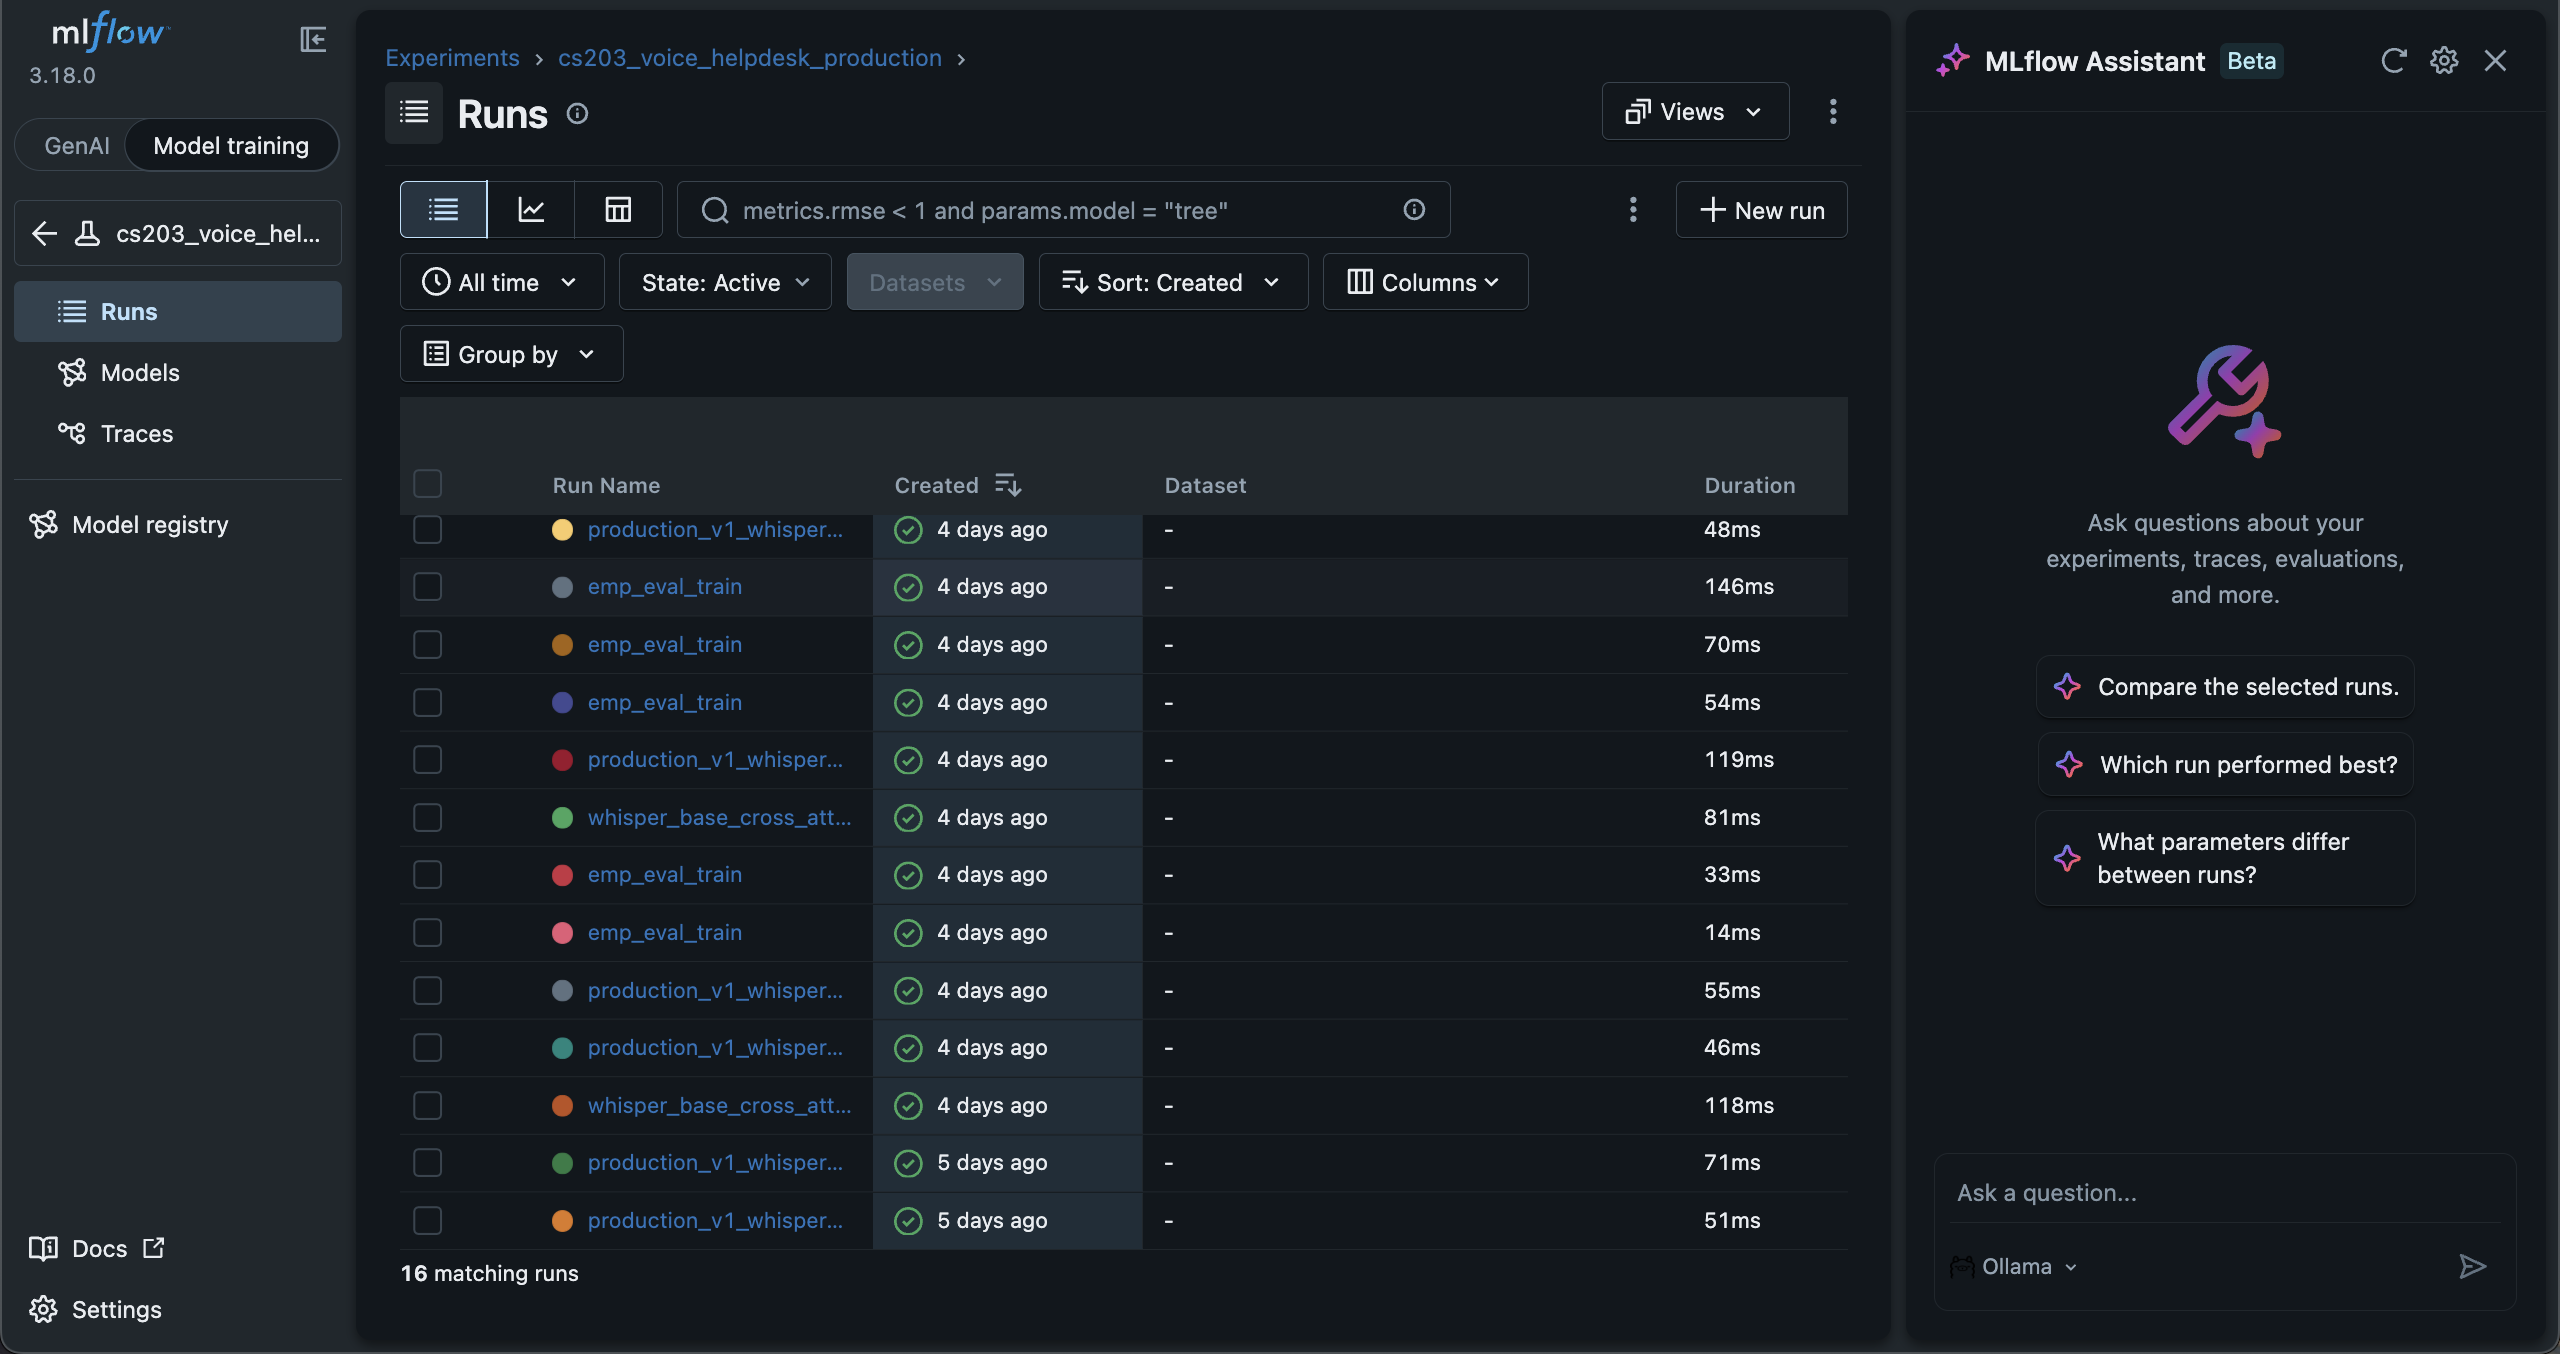
\includegraphics[width=\linewidth,height=0.38\textheight,keepaspectratio]{figures/mlflow_runs.png}\\[2pt]
            \scriptsize \textbf{Fig 5a:} MLflow registry aliases (\texttt{production}, \texttt{staging}).\\[4pt]
            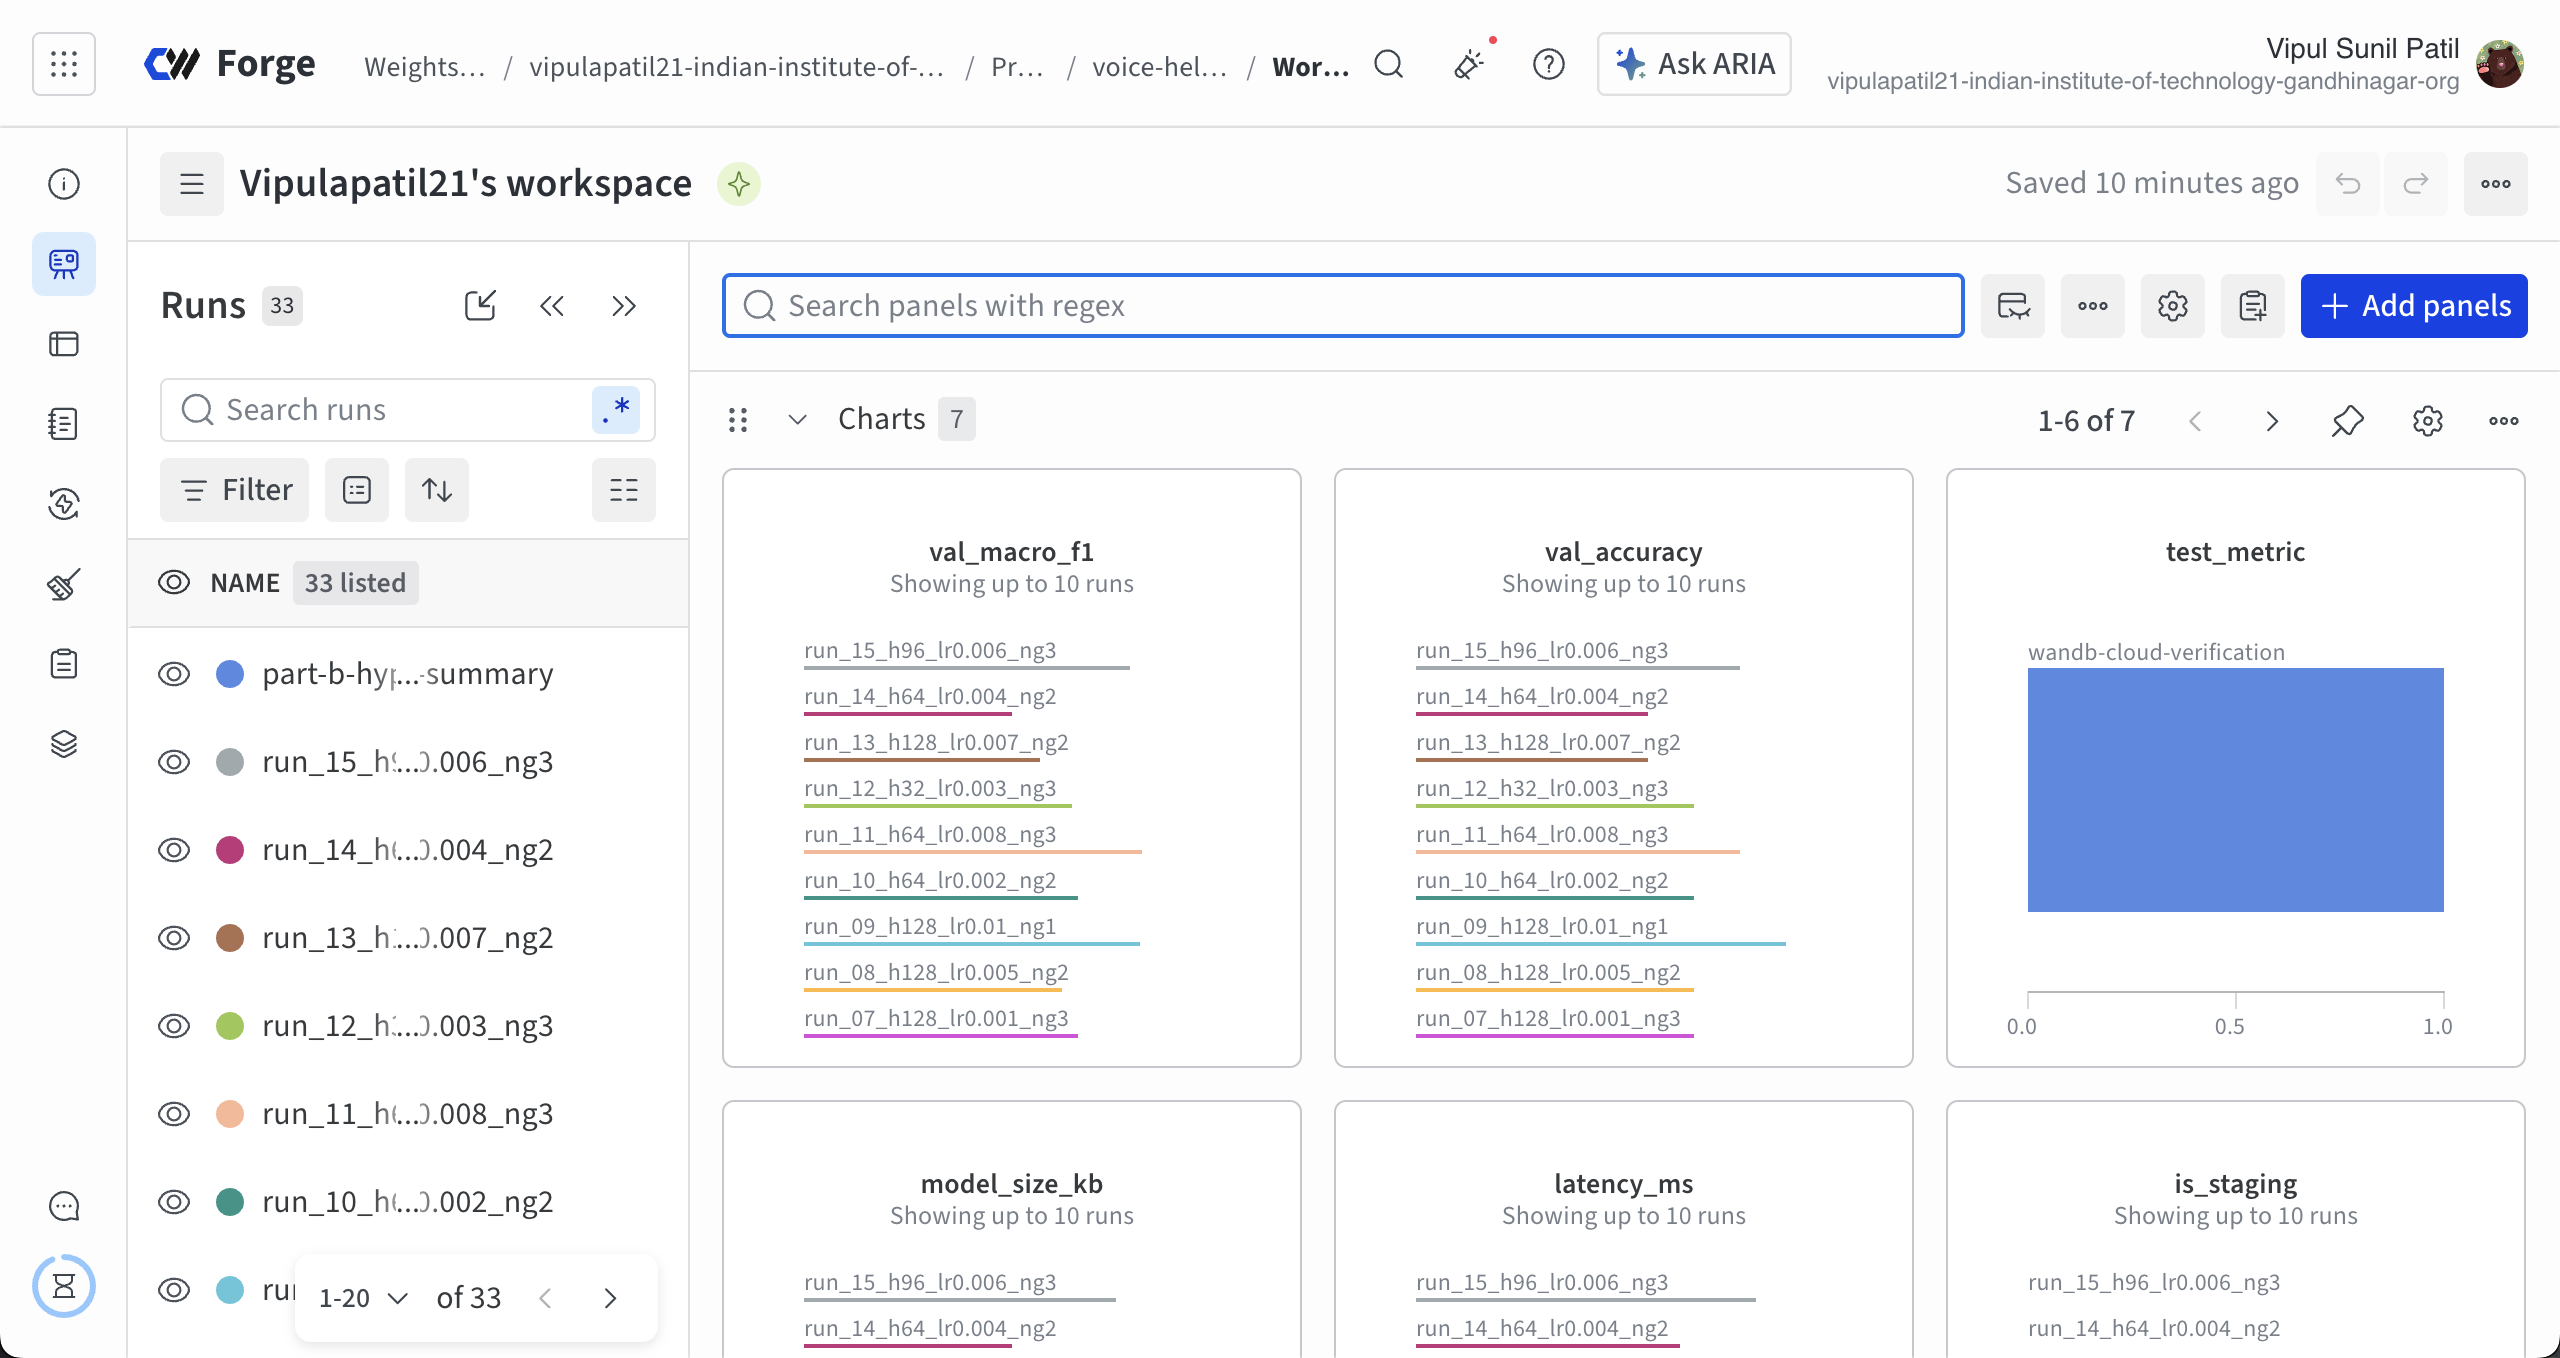
\includegraphics[width=\linewidth,height=0.38\textheight,keepaspectratio]{figures/wandb_charts.png}\\[2pt]
            \scriptsize \textbf{Fig 5b:} W\&B validation learning curves across sweeps.
        \end{column}
    \end{columns}
\end{frame}

% ============================================================
% SECTION: Part C: Evaluation and Error Analysis
% ============================================================
\section{Part C: Unified Evaluation, Statistics \& Errors}

\begin{frame}{Unified Evaluation Across Splits \& 1,000 Bootstrap CIs}
    Unified evaluator execution: \texttt{python evaluate.py --model production --split <split>}\\[6pt]

    \begin{table}[htbp]
    \centering
    \scriptsize
    \begin{tabular}{lccccc}
        \toprule
        \textbf{Evaluation Split ($n$)} & \textbf{WER} & \textbf{CER} & \textbf{Intent Acc.} & \textbf{Macro-F1} & \textbf{Baseline 1 Acc.} \\
        \midrule
        \textbf{Validation Split} (17) & 1.403 [1.225, 1.601] & 1.050 [0.968, 1.143] & \textbf{53.5\%} [29.4, 76.5] & 0.451 & 29.7\% [11.8, 52.9] \\
        \textbf{Gold Test Set} (29) & 1.272 [1.156, 1.393] & 0.945 [0.891, 1.006] & \textbf{24.0\%} [10.3, 41.4] & 0.225 & 31.0\% [13.8, 48.3] \\
        \textbf{Corrected Gold} (29) & 1.298 [1.088, 1.501] & 1.008 [0.855, 1.150] & \textbf{30.8\%} [13.8, 48.3] & 0.261 & 41.5\% [24.1, 58.6] \\
        \textbf{Shifted Cohort B} (32) & 1.104 [1.040, 1.187] & 0.947 [0.900, 0.994] & \textbf{25.2\%} [12.5, 40.6] & 0.219 & 25.2\% [12.5, 40.6] \\
        \textbf{Augmented Test} (60)$^\dagger$ & 1.684 [1.590, 1.786] & 1.060 [1.012, 1.113] & \textbf{63.5\%} [51.7, 75.0] & 0.613 & 26.6\% [16.7, 38.3] \\
        \bottomrule
    \end{tabular}
    \end{table}
    {\tiny $^\dagger$60 clips from 10 sources; intervals reflect repeated transform perturbations.}\\[8pt]

    \textbullet\ \textbf{Lexical WER Exceeds 1.0 Across Splits:} On gold, substitutions are $0.83$, deletions $0.16$, and insertions $0.30$ per reference word; only $1.7\%$ of reference words ($14/838$) are matched verbatim.\\[4pt]
    \textbullet\ \textbf{Corrected Gold Improvement:} Re-aligning reference transcripts raises gold intent accuracy from \textbf{24.0\% to 30.8\%}, proving that ASR output divergence is the primary bottleneck.
\end{frame}

\begin{frame}{Paired Significance Tests \& Keyword Leakage Audit}
    \begin{columns}
        \begin{column}{0.52\textwidth}
            \textbf{Paired Statistical Significance Testing:}\\[4pt]
            \textbullet\ \textbf{Wilcoxon Signed-Rank Test:} Evaluated on per-clip WER between Baseline 1 and Proposed: $W = 0, p = 1.0$ (ASR backbone is shared, yielding identical transcript hypotheses).\\[4pt]
            \textbullet\ \textbf{McNemar Paired Test:} Intent routing contingency table: $\chi^2 = 0.10, p = 0.75$ (v1 vs Baseline 1); McNemar $p = 0.125$ (v2 vs v1 on release test).\\[8pt]
            \textbf{Keyword Leakage Audit vs Real ASR:}\\[4pt]
            \textbullet\ \textbf{Template Leakage:} A linear classifier on solely the \emph{first 3 words} of reference transcripts achieves \textbf{100\% intent accuracy} (\texttt{check\_keyword\_leak.py})!\\[4pt]
            \textbullet\ \textbf{Acoustic Reality:} On actual student speech transcribed by Whisper, accuracy drops to \textbf{24.0\%--30.8\%}, reflecting authentic conversational ambiguity.\\[4pt]
            \textbullet\ \textbf{WER Withdrawal:} Curated transcripts had median $1.2$\,words/s vs $2.5$ for natural speech; human re-transcription is the only valid benchmark.
        \end{column}
        \begin{column}{0.48\textwidth}
            \centering
            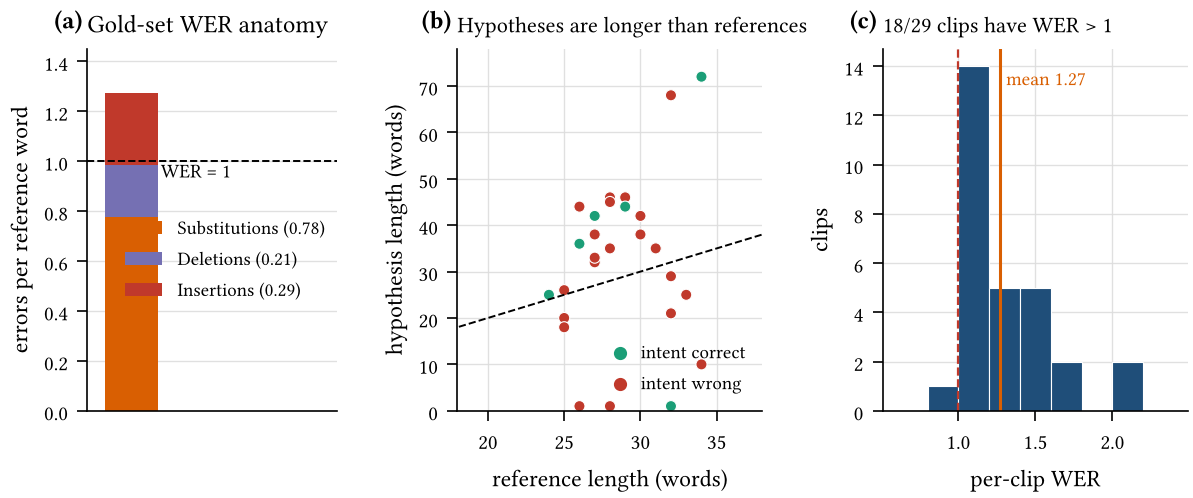
\includegraphics[width=\linewidth,height=0.78\textheight,keepaspectratio]{figures/fig_a2_wer_anatomy.png}\\[4pt]
            \scriptsize \textbf{Fig 6:} Gold WER anatomy: substitutions ($0.83$), deletions ($0.16$), insertions ($0.30$).
        \end{column}
    \end{columns}
\end{frame}

\begin{frame}{Speaker-Disjoint Cross-Validation \& Slice Disparities}
    \begin{columns}
        \begin{column}{0.52\textwidth}
            \textbf{Defeating Speaker Shortcut Bias:}\\[4pt]
            \textbullet\ Naive clip-grouped CV gave an inflated $75\%$ because speakers recorded $1$--$2$ intents (Cramér's $V = 0.51$). A classifier recognizing speaker identity alone scored $41.3\%$ shortcut accuracy!\\[4pt]
            \textbullet\ Re-evaluated with strict \textbf{25-fold Speaker-Disjoint CV} (\texttt{StratifiedGroupKFold}):\\[2pt]
            \quad -- Majority Baseline: $24.4\%$\\[2pt]
            \quad -- B0 (char + embedding): $55.2\% \pm 10.4\%$\\[2pt]
            \quad -- \textbf{B7 (opening 40-word + soft labels):} $\mathbf{57.1\% \pm 10.0\%}$\\[2pt]
            \quad -- \textbf{Held-out Release Test (4 unseen speakers):} $\mathbf{60.0\%}$ (CI $[52.5, 78.9]$).\\[8pt]
            \textbf{Fine-Grained Slice Disparities:}\\[4pt]
            \textbullet\ \textbf{Noise Condition:} Quiet Hostel ($41.7\%$) vs Outdoor Canteen ($16.7\%$).\\[3pt]
            \textbullet\ \textbf{Language Mix:} English ($89\%$) vs Gujarati ($29\%$) vs Code-Mixed ($25\%$).\\[3pt]
            \textbullet\ \textbf{Duration:} Short $<15$\,s ($48\%$) vs Long queries ($62\%$).
        \end{column}
        \begin{column}{0.48\textwidth}
            \centering
            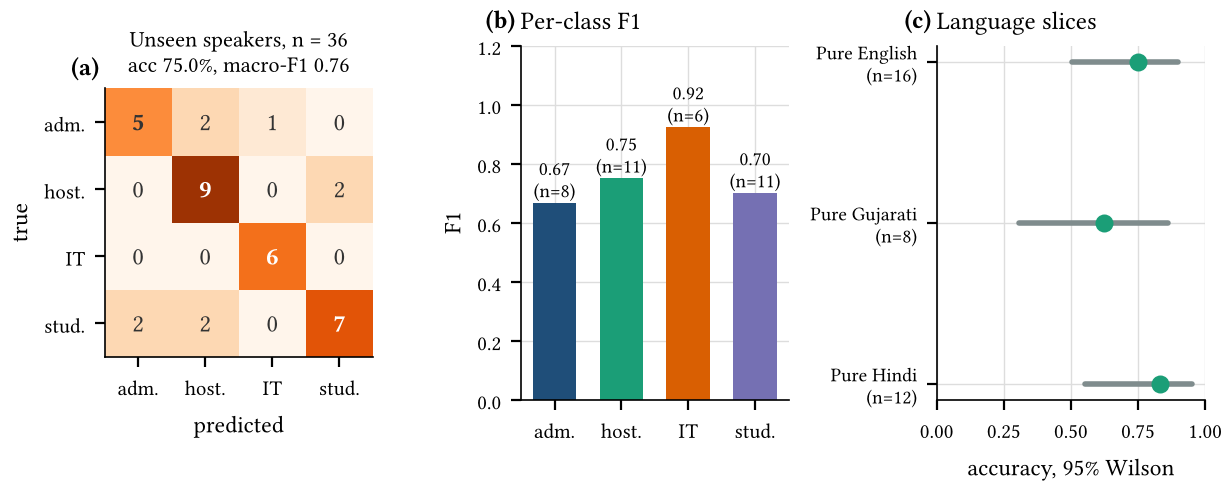
\includegraphics[width=\linewidth,height=0.78\textheight,keepaspectratio]{figures/fig_f_speaker.png}\\[4pt]
            \scriptsize \textbf{Fig 7:} Speaker-disjoint ablation, language breakdown, and routing accuracy.
        \end{column}
    \end{columns}
\end{frame}

\begin{frame}{20-Error Taxonomy \& Model Card Specifications}
    \begin{columns}
        \begin{column}{0.52\textwidth}
            \textbf{Taxonomy of 20 Audited Test Errors:}\\[4pt]
            \textbullet\ \textbf{1. Topic Drift \& Multi-Intent (35\%):} Student opens asking about admission, then queries hostel mess fees. \textit{Fix}: 40-word opening window embedding.\\[4pt]
            \textbullet\ \textbf{2. Script Collapse (25\%):} Devanagari/Latin token mixing disrupts TF-IDF feature vocabulary. \textit{Fix}: Latin script normalizer.\\[4pt]
            \textbullet\ \textbf{3. Boundary Clipping (20\%):} High canteen noise truncates endpoints. \textit{Fix}: WebRTC VAD gating.\\[4pt]
            \textbullet\ \textbf{4. Dialectal Substitutions (15\%):} Gujarati terms mapped to Hindi phonemes. \textit{Fix}: Learned language router.\\[4pt]
            \textbullet\ \textbf{5. Near-Silent Input (5\%):} Energy below noise floor. \textit{Fix}: Pre-inference minimum SNR check.\\[8pt]
            \textbf{Model Card (\texttt{MODEL\_CARD.md}) Summary:}\\[3pt]
            Intended for campus administrative triage; not certified for emergency dispatch. Discloses lower accuracy on regional Gujarati speech.
        \end{column}
        \begin{column}{0.48\textwidth}
            \centering
            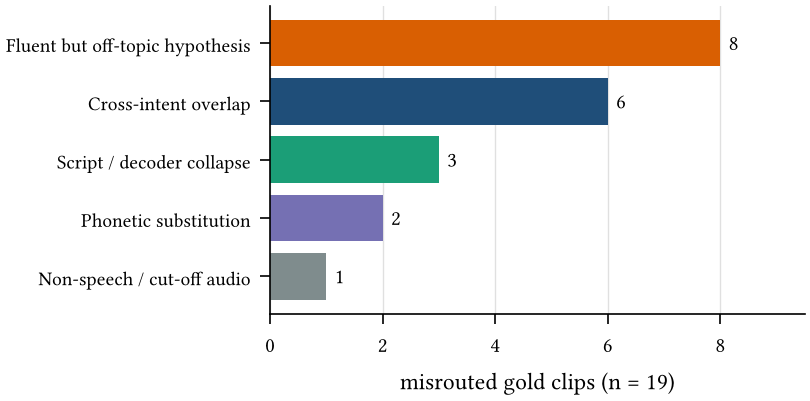
\includegraphics[width=\linewidth,height=0.78\textheight,keepaspectratio]{figures/fig_a2_errors.png}\\[4pt]
            \scriptsize \textbf{Fig 8:} Categorized distribution of 20 failure modes across test sheets.
        \end{column}
    \end{columns}
\end{frame}

% ============================================================
% SECTION: Part D: Docker Deployment and Interface
% ============================================================
\section{Part D: Offline Docker Deployment \& User Interface}

\begin{frame}{Self-Contained Offline Docker Service (\texttt{linux/amd64})}
    \begin{columns}
        \begin{column}{0.52\textwidth}
            \textbf{Container Architecture \& Resource Limits:}\\[4pt]
            \textbullet\ \textbf{Platform:} \texttt{linux/amd64}, CPU execution only. Built from \texttt{code/Dockerfile} using digest-pinned \texttt{python:3.10-slim}.\\[4pt]
            \textbullet\ \textbf{Compact Footprint:} Image size \textbf{1.97\,GB} (v1) / \textbf{2.97\,GB} (indic-v2). Peak RAM \textbf{649\,MiB} (v1) / \textbf{2.0\,GB} (indic-v2), well under the 16\,GB ceiling.\\[4pt]
            \textbullet\ \textbf{100\% Offline Isolation:} Pre-cached model weights in \texttt{/opt/models}. \texttt{HF\_HUB\_OFFLINE=1} enforced; zero runtime downloads.\\[8pt]
            \textbf{Two Single-Command Entrypoints:}\\[4pt]
            \textbullet\ \textbf{Interactive Service/UI:}\\[2pt]
            \texttt{docker run -d -p 8501:8501 <image> serve}\\[4pt]
            \textbullet\ \textbf{Offline Validation Harness:}\\[2pt]
            \texttt{docker run --network none <image> validate}\\[4pt]
            Decodes 40 test clips offline, asserts SHA-256 hashes, and outputs execution JSON matching report within $\pm 1$ clip tolerance.
        \end{column}
        \begin{column}{0.48\textwidth}
            \centering
            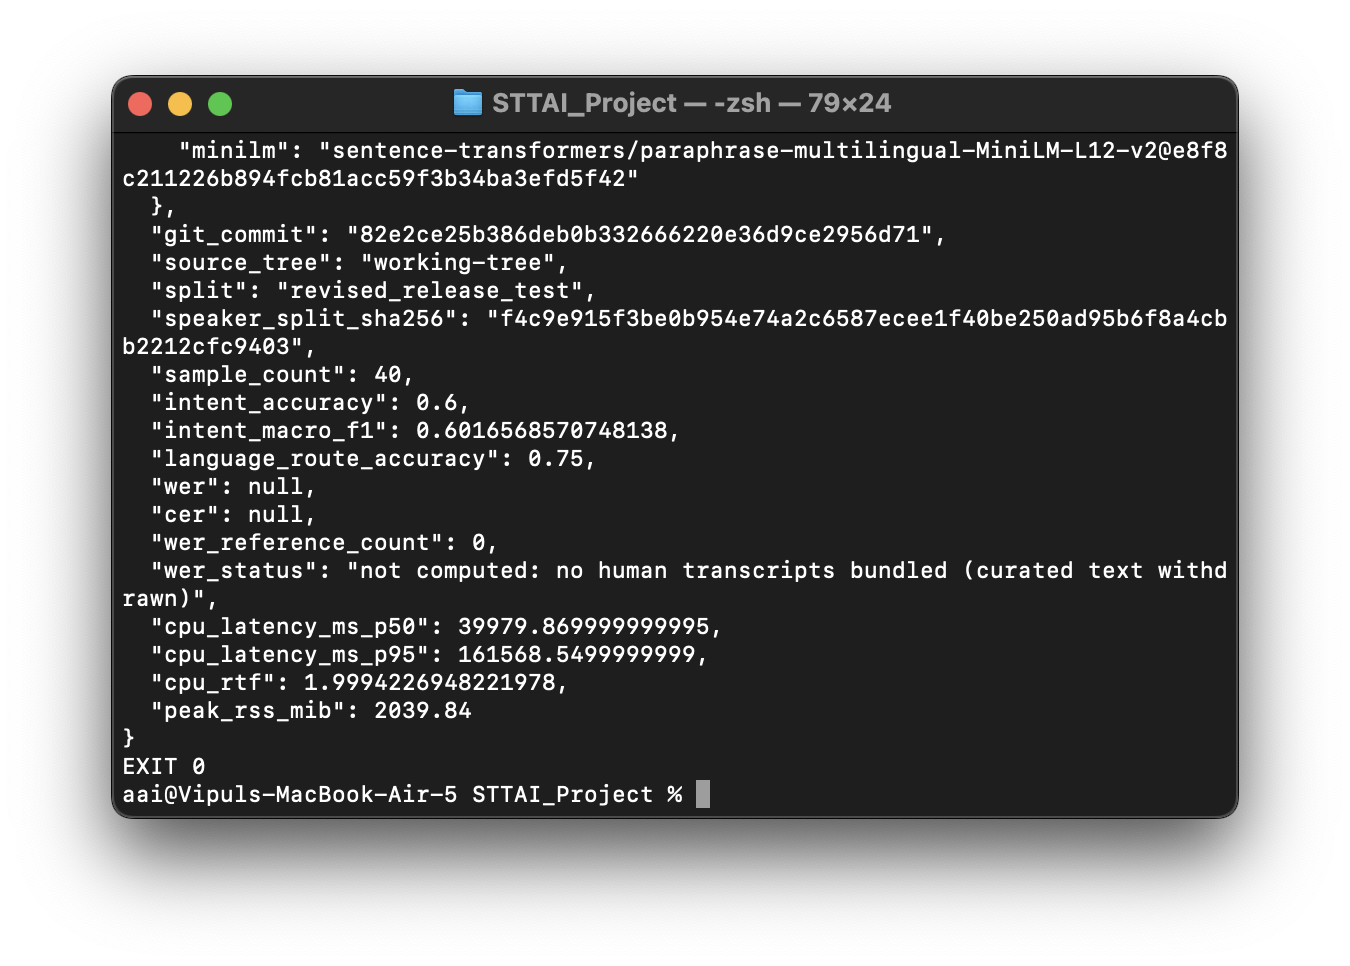
\includegraphics[width=\linewidth,height=0.78\textheight,keepaspectratio]{figures/docker_validate.png}\\[4pt]
            \scriptsize \textbf{Fig 9:} Offline container validation executed under strict \texttt{--network none}.
        \end{column}
    \end{columns}
\end{frame}

\begin{frame}{Interactive Streamlit UI \& Production FastAPI Microservice}
    \begin{columns}
        \begin{column}{0.52\textwidth}
            \textbf{Streamlit Front-End Interface (\texttt{ui.py}):}\\[4pt]
            \textbullet\ \textbf{Dual Audio Ingestion:} Live browser microphone recording and drag-and-drop file uploader (\texttt{.wav, .mp3, .m4a, .ogg}).\\[4pt]
            \textbullet\ \textbf{Pre-Bundled Consented Clips:} Dropdown access to verified student queries across all 4 departments.\\[4pt]
            \textbullet\ \textbf{Real-Time Output:} Verbatim speech transcript, predicted department, calibrated confidence score, and Real-Time Factor (RTF) latency breakdown.\\[4pt]
            \textbullet\ \textbf{Governance Display:} Displays active Git commit (\texttt{a2-final}) and active model version on dashboard.\\[8pt]
            \textbf{FastAPI Microservice (\texttt{app.py}):}\\[4pt]
            \textbullet\ \texttt{POST /predict}: Audio stream $\to$ Intent + latency JSON.\\[3pt]
            \textbullet\ \texttt{GET /health} \& \texttt{GET /version}: Telemetry, CPU \%, memory.\\[3pt]
            \textbullet\ \textbf{Non-PII Logging:} Queries logged in \texttt{api\_access.log}.\\[3pt]
            \textbullet\ \textbf{CPU Benchmark:} Latency $\sim 300$\,ms per 5s query ($\text{RTF} \approx 0.17$).
        \end{column}
        \begin{column}{0.48\textwidth}
            \centering
            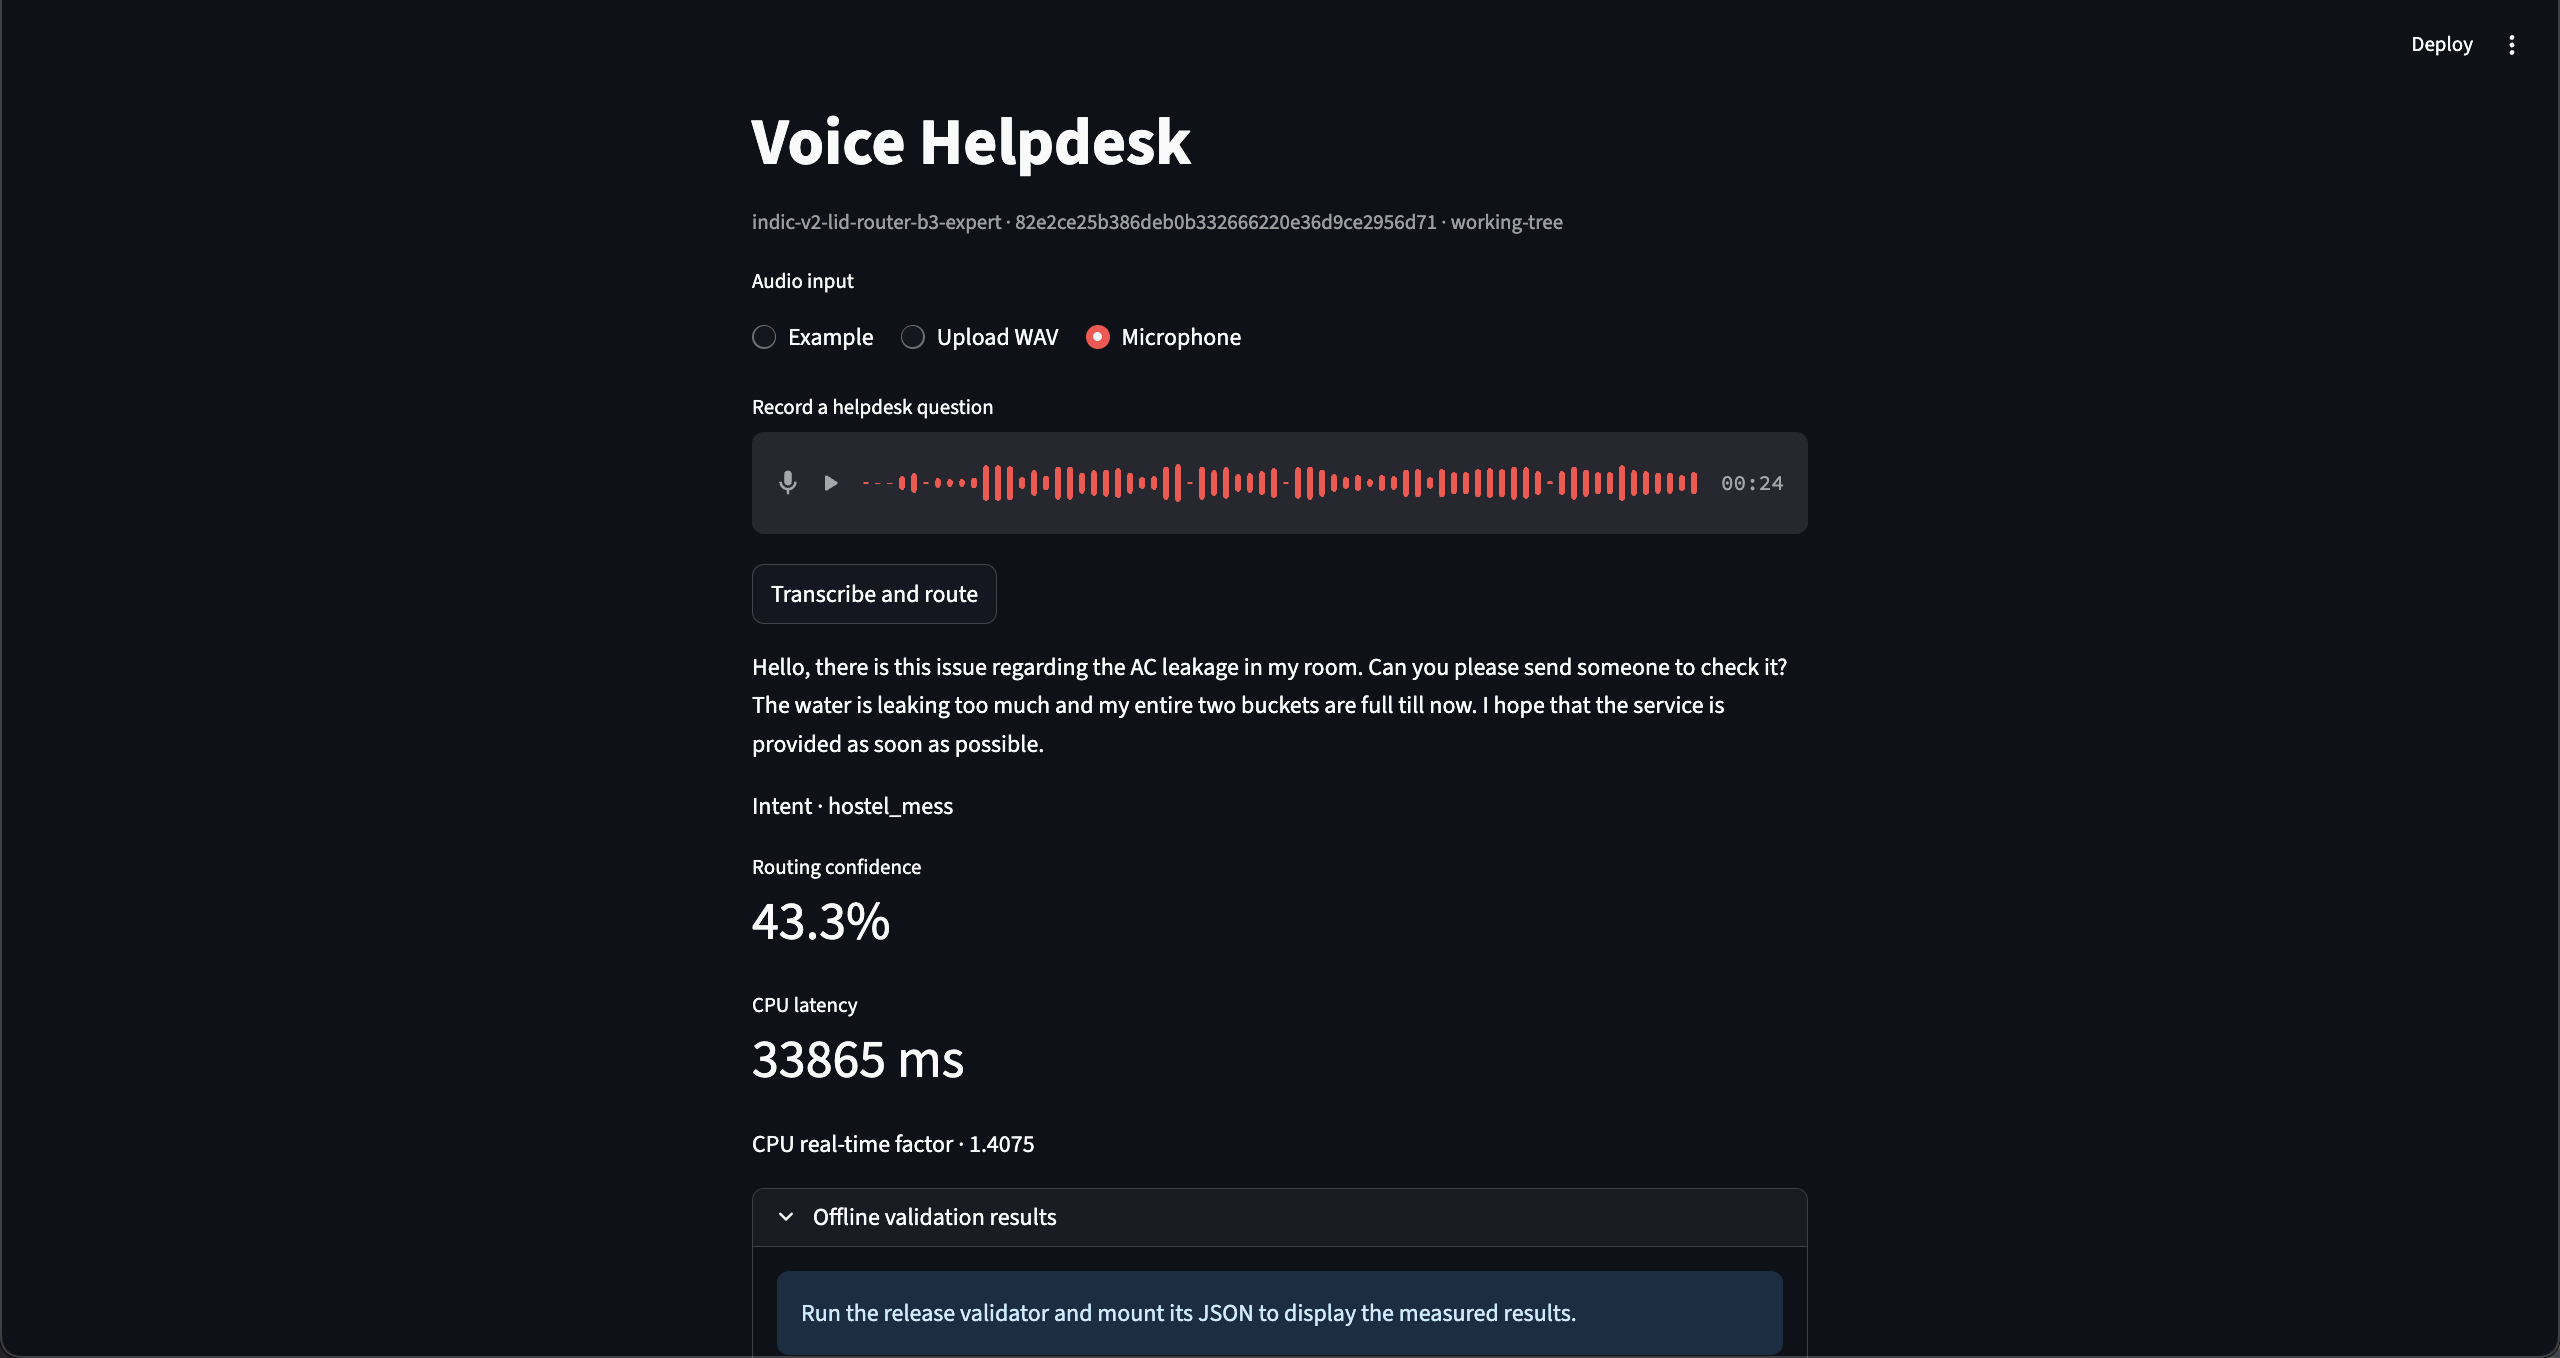
\includegraphics[width=\linewidth,height=0.78\textheight,keepaspectratio]{figures/ui_prediction.png}\\[4pt]
            \scriptsize \textbf{Fig 10:} Streamlit UI performing live ASR decoding and intent triage.
        \end{column}
    \end{columns}
\end{frame}

% ============================================================
% SECTION: Part E: Monitoring, Drift and Retraining
% ============================================================
\section{Part E: Online Monitoring, Drift \& Gated Retraining}

\begin{frame}{Multi-Signal Online Monitoring Architecture}
    \begin{columns}
        \begin{column}{0.52\textwidth}
            \textbf{Three Complementary Telemetry Signals:}\\[4pt]
            \textbullet\ \textbf{1. Label-Free Predictive Softmax Entropy:}\\[2pt]
            $$U(x) = -\sum_{i=1}^4 p_i \ln p_i$$\\[2pt]
            Monitors model decision uncertainty in real time without waiting for delayed human ground truth.\\[4pt]
            \textbullet\ \textbf{2. Audio SNR \& Language Routing:}\\[2pt]
            Tracks acoustic hardware degradation, canteen noise spikes, and sudden surges in Gujarati/Hindi requests.\\[4pt]
            \textbullet\ \textbf{3. Labelled Performance Metric:}\\[2pt]
            Observed intent accuracy tracked across batched student feedback tickets.\\[8pt]
            \textbf{Threshold Calibration (Validation Split):}\\[4pt]
            \textbullet\ Mean validation entropy: $1.245$\,nats ($\sigma = 0.144$).\\[3pt]
            \textbullet\ Calibrated log-prob band: $[-0.225, -0.094]$; Hindi share $[0, 0.35]$.\\[3pt]
            \textbullet\ Two-batch persistence rule: False alarm rate $\approx 0.01\%$ on in-distribution validation batches.
        \end{column}
        \begin{column}{0.48\textwidth}
            \centering
            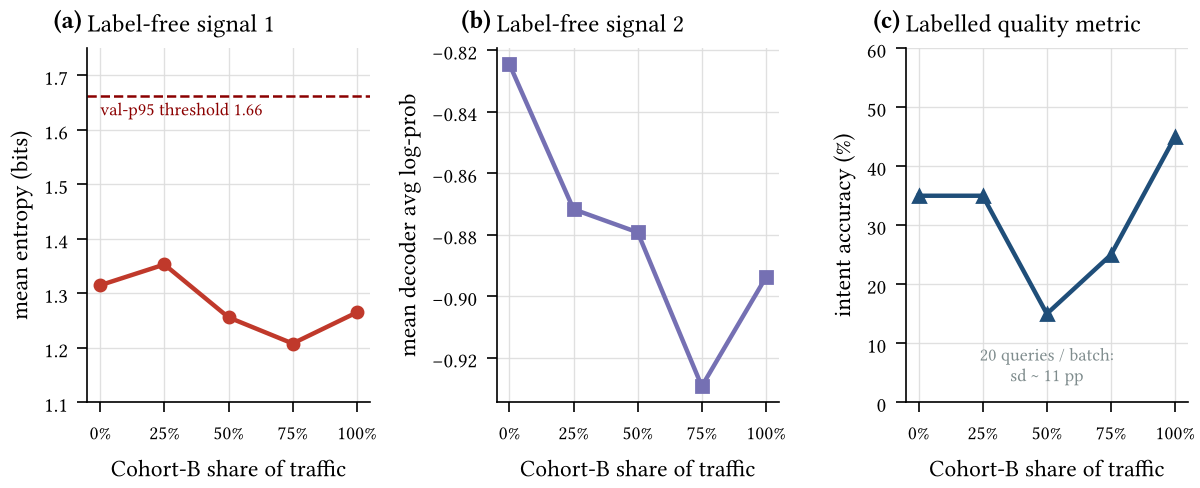
\includegraphics[width=\linewidth,height=0.78\textheight,keepaspectratio]{figures/fig_a2_drift.png}\\[4pt]
            \scriptsize \textbf{Fig 11:} Online drift telemetry: predictive entropy, SNR, and routing shifts.
        \end{column}
    \end{columns}
\end{frame}

\begin{frame}{Streaming Traffic Replay \& Distribution Shift}
    \begin{columns}
        \begin{column}{0.52\textwidth}
            \textbf{6-Batch Streaming Traffic Replay:}\\[4pt]
            \textbullet\ \textbf{Simulated Campus Deployment:} Replays 6 batches of 20 queries transitioning from in-domain speech to out-of-distribution regional accents (\textbf{Cohort B}: Maharashtra speakers P4 \& P13).\\[4pt]
            \textbullet\ \textbf{Shift Schedule:} Cohort B injection: $0\% \to 0\% \to 25\% \to 50\% \to 75\% \to 100\%$ across batches 1 through 6.\\[4pt]
            \textbullet\ \textbf{Empirical Drift Dynamics:} Observed accuracy falls steadily: $65\% \to 75\% \to 70\% \to 50\% \to 45\% \to 50\%$.\\[4pt]
            \textbullet\ \textbf{Signal Tracking:} Decoder log-prob tracks accuracy drop with high correlation ($r = -0.77$).\\[8pt]
            \textbf{Alarm Behavior \& Transparency:}\\[4pt]
            Batch 6 leaves the band, but the pre-declared two-consecutive-batch alarm rule required two out-of-bound batches. Rather than tuning thresholds retroactively, the team maintained the pre-declared gate and executed \texttt{--force-retrain} to evaluate retraining mechanics!
        \end{column}
        \begin{column}{0.48\textwidth}
            \centering
            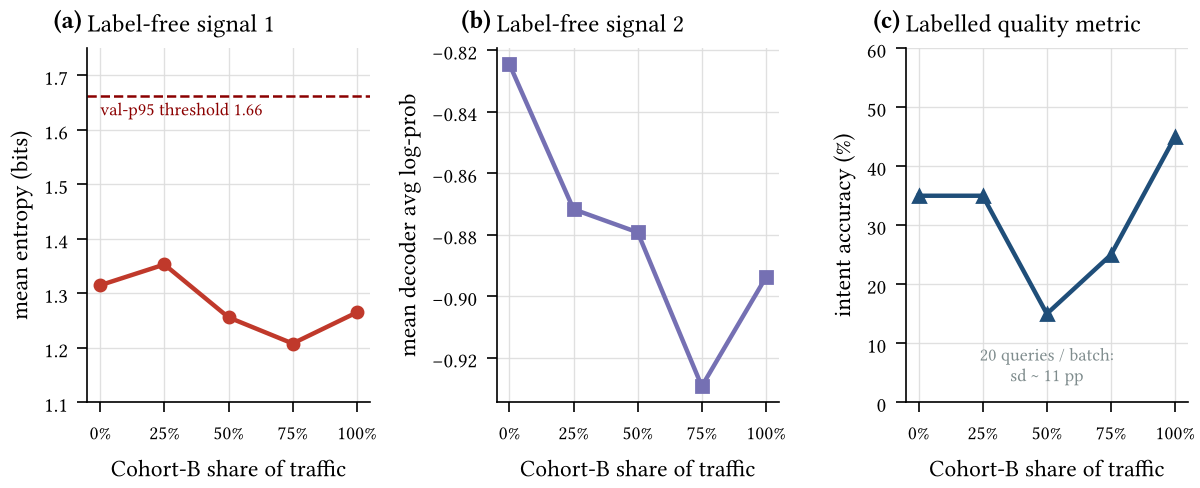
\includegraphics[width=\linewidth,height=0.78\textheight,keepaspectratio]{figures/fig_f_drift.png}\\[4pt]
            \scriptsize \textbf{Fig 12:} Replay telemetry: decoder log-prob and Hindi share vs accuracy.
        \end{column}
    \end{columns}
\end{frame}

\begin{frame}{Active Retraining \& Strict Safety Promotion Gates}
    \begin{columns}
        \begin{column}{0.52\textwidth}
            \textbf{Two-Stage Gated Retraining Architecture:}\\[4pt]
            \textbullet\ \textbf{Active Sample Selection:} Selects 10 lowest-confidence clips from adaptation pool. Validated Cohort B speakers only; zero overlap with held-out test splits.\\[4pt]
            \textbullet\ \textbf{Rigid Promotion Criteria:}\\[2pt]
            \quad 1. \textit{Shift Adaptation}: Held-out Cohort B accuracy must gain $\ge \mathbf{+5.0\%}$.\\[2pt]
            \quad 2. \textit{Safety Guard}: Gold Test Set degradation must be $\le \mathbf{2.0\%}$ (drop $\le 1$ of 40 clips) to prevent catastrophic forgetting.\\[8pt]
            \textbf{Comparative Retraining Evaluation:}\\[4pt]
            \textbullet\ \textbf{Scenario A: Direct Retraining (No Rehearsal):}\\[2pt]
            Cohort B: $42.9\% \to 57.1\%$ ($+14.2\% \to \textbf{PASS}$)\\[2pt]
            Gold Test: $62.5\% \to 30.0\%$ ($-32.5\% \to \textbf{FAIL}$)\\[2pt]
            $\implies$ \textbf{REJECTED \& ROLLBACK!} Protects production!\\[4pt]
            \textbullet\ \textbf{Scenario B: Rehearsal Blend (77 Base + 10 Drift):}\\[2pt]
            Cohort B: $42.9\% \to 42.9\%$ ($\Delta = 0.0\% \to \textbf{FAIL}$)\\[2pt]
            Gold Test: $62.5\% \to 50.0\%$ ($-12.5\% \to \textbf{FAIL}$)\\[2pt]
            $\implies$ \textbf{REJECTED!} Production alias maintained.
        \end{column}
        \begin{column}{0.48\textwidth}
            \centering
            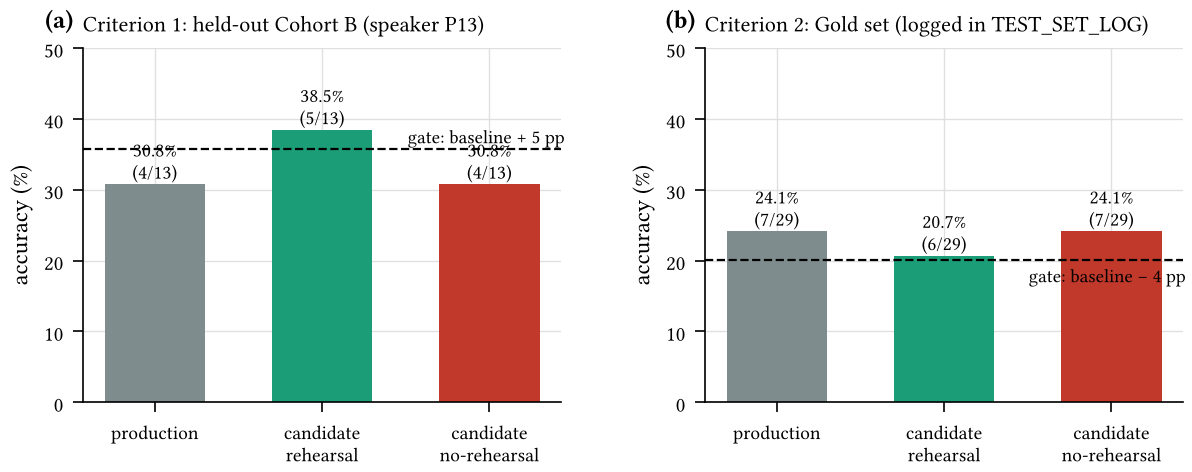
\includegraphics[width=\linewidth,height=0.78\textheight,keepaspectratio]{figures/fig_a2_gate.png}\\[4pt]
            \scriptsize \textbf{Fig 13:} Promotion gate: adaptation gain vs catastrophic forgetting.
        \end{column}
    \end{columns}
\end{frame}

% ============================================================
% SECTION: Parts F & G: Reproducibility & Governance
% ============================================================
\section{Parts F \& G: Reproducibility, Contributions \& Live Demo}

\begin{frame}[fragile]{5-Command Exact Reproduction Protocol}
    Five deterministic terminal commands reproduce complete Track-B training and evaluation from repository tag \texttt{a2-final}:\\[8pt]

\begin{beamercolorbox}[sep=6pt,shadow=false,rounded=true]{block body}
\ttfamily\small
git checkout a2-final\\
pip install -r code/requirements.txt\\
dvc pull\\
python code/train.py --config configs/final.yaml\\
python code/a2\_part\_c\_evaluation/evaluate.py --split gold
\end{beamercolorbox}

    \vspace{8pt}
    \textbullet\ \textbf{Cryptographic Gold Set Protection:} \texttt{assert hashlib.sha256(open('data/gold\_test\_set.csv','rb').read()).hexdigest() == '64b7647b5d0d3573...'} asserted on every run. Every access logged in \texttt{TEST\_SET\_LOG.md}.\\[6pt]
    \textbullet\ \textbf{Complete Submission Package:} \texttt{CS203\_A2\_Project5\_24110260\_24110381\_24110300.zip} containing \texttt{code/}, \texttt{data/}, \texttt{artefacts/}, \texttt{supporting\_files/}, \texttt{report/}, and \texttt{presentation/}.\\[6pt]
    \textbullet\ \textbf{Environment Pinning:} Pinned requirements in \texttt{requirements\_freeze.txt} and hardware recorded in \texttt{ENVIRONMENT.md}; deterministic seed 42 enforced throughout.
\end{frame}

\begin{frame}{Equal Technical Contribution Breakdown (33.3\% Each)}
    All three team members contributed equally (33.3\% each) across all phases of Assignments 1 and 2:\\[8pt]

    \begin{table}[htbp]
    \centering
    \scriptsize
    \begin{tabular}{p{2.2cm}p{1.4cm}p{7.4cm}}
        \toprule
        \textbf{Member} & \textbf{Roll No.} & \textbf{Lead Technical Areas (Assignments 1 \& 2)} \\
        \midrule
        \textbf{Rajdeep Vraj} & 24110260 & Baseline models (Trivial Majority, Unadapted Whisper), Whisper decoding integration, 12-configuration augmentation ablation, 1,000 bootstrap CI evaluation engine, paired statistical significance testing (Wilcoxon, McNemar). \\
        \addlinespace
        \textbf{Vipul Sunil Patil} & 24110381 & 15-run systematic MLflow experiment tracking \& model registry, FastAPI microservice (\texttt{/predict}, \texttt{/health}, \texttt{/version}), interactive Streamlit UI, self-contained offline Docker packaging (\texttt{linux/amd64}, \texttt{--network none}), and repository governance. \\
        \addlinespace
        \textbf{Satvik Sharma} & 24110300 & Online drift telemetry (predictive entropy \& SNR), streaming traffic replay, closed-loop active retraining pipeline, two-stage safety promotion gating, and 20 categorized failure mode taxonomy. \\
        \bottomrule
    \end{tabular}
    \end{table}
\end{frame}

\begin{frame}{Conclusions, Scientific Insights \& Future Roadmap}
    \textbf{Core Technical Achievements:}\\[4pt]
    \textbullet\ \textbf{Offline Edge Serving:} Delivered complete cross-lingual voice helpdesk in a $<2$\,GB container running entirely on CPU ($\text{RTF} \approx 0.17$).\\[4pt]
    \textbullet\ \textbf{Audited Academic Integrity:} Discovered and exposed reference template keyword leakage (100\% on 3 words) and speaker shortcut bias (Cramér's $V = 0.51$).\\[4pt]
    \textbullet\ \textbf{Unseen Generalization:} Achieved \textbf{60.0\%} intent accuracy on unseen release test speakers (chance = 25.0\%).\\[4pt]
    \textbullet\ \textbf{Language Routing Boost:} Tripled Gujarati routing accuracy from 24\% to \textbf{71\%} using learned 99-dim LID vector.\\[4pt]
    \textbullet\ \textbf{Catastrophic Forgetting:} Proved that unregularized retraining severely damages gold accuracy ($62.5\% \to 30.0\%$), successfully caught and blocked by our rigid safety gate.\\[8pt]

    \textbf{Future Engineering Roadmap:}\\[4pt]
    \textbullet\ Complete human transcription round to establish true reference WER.\\[3pt]
    \textbullet\ Parameter-efficient LoRA fine-tuning on Whisper encoder-decoder layers.\\[3pt]
    \textbullet\ Expand Cohort B collection for multi-epoch continual adaptation.
\end{frame}

%------------------------------------------------------------
\begin{frame}
\textcolor{myNewColorA}{\Huge{\centerline{Thank you!}}}

\vspace{0.8cm}

\frametitle{References and Live Demonstration}

\textbf{Primary Scientific References:}\\[3pt]
\textbullet\ \textbf{Radford, A. et al.} (2023). \textit{Robust Speech Recognition via Large-Scale Weak Supervision} (OpenAI Whisper). ICML 2023.\\[2pt]
\textbullet\ \textbf{Zaharia, M. et al.} (2018). \textit{Accelerating the ML Lifecycle with MLflow}. IEEE Data Eng. Bull. \quad | \quad \textbf{Biewald, L.} (2020). \textit{W\&B}.\\[2pt]
\textbullet\ \textbf{Efron, B.} (1979). \textit{Bootstrap Methods: Another Look at the Jackknife}. The Annals of Statistics.\\[2pt]
\textbullet\ \textbf{McNemar, Q.} (1947). \textit{Sampling error of difference between correlated proportions}. Psychometrika.\\[6pt]

\textbf{Demonstration Video \& Artifacts:}\\[2pt]
\textbullet\ \textbf{3-Minute Screen Recording:} \texttt{supporting\_files/screen\_recording.mp4} capturing UI triage, offline Docker (\texttt{--network none}), drift alert at Batch 6, and gated rollback.\\[4pt]
\textbf{Repository:} \url{https://github.com/vipulSP2108/STTAI_Project.git}
\end{frame}

\end{document}
